\section{Introducción}

  Un \emph{alto horno} es un horno cilíndrico en cuyo interior se realiza la fusión de metales a temperaturas muy elevadas. Dado que las paredes del horno se encuentran sometidas a estas condiciones extremas, resulta importante conocer, por cuestiones de seguridad, si su estructura corre riesgo de colapsar a causa del calor. Este problema físico es el que se pretende resolver, a través de un modelo matemático, en el transcurso de este trabajo.

  \begin{figure}[h]
    \centering
    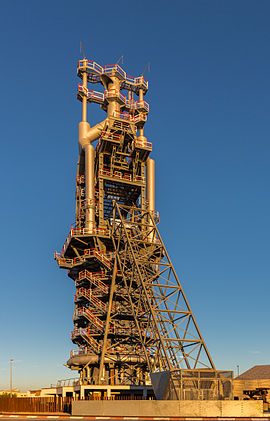
\includegraphics[width=4cm]{imagenes/altoHorno.jpg}
    \caption{Alto horno.} \label{fig:alto-horno}
  \end{figure}

  Se considerará una sección horizontal del horno. La temperatura en el interior del horno es constante y conocida; además, se cuenta con sensores ubicados a intervalos regulares en el exterior de la pared, que proporcionan información sobre la temperatura (variable) de la misma. A partir de esta información, se pretende en primer lugar estimar el valor de la temperatura en los puntos correspondientes al interior de la pared.

  Para encarar el problema de forma computacional, su dominio será discretizado mediante un modelo matemático; es decir, se seleccionará un conjunto finito de puntos del mismo en el que calcular los resultados. Esto permitirá obtener los mismos a través de la resolución de un sistema de ecuaciones lineales. Por este motivo, serán de interés los métodos que permitan encontrar soluciones a este tipo de sistemas. Se utilizarán dos de ellos: el método de Eliminación Gaussiana y el de Factorización LU.

  Luego, teniendo en cuenta los resultados obtenidos, se buscará interpretarlos para evaluar la peligrosidad de la estructura. En particular, se considerará una temperatura crítica, con el objetivo de calcular la posición de la isoterma correspondiente a la misma, es decir, el conjunto de puntos de la pared que se encuentran a dicha temperatura. La cercanía de esta isoterma a la pared externa del horno será la que determinará la existencia de una situación de riesgo de colapso de la estructura. En este sentido, se estudiará también la elaboración de un criterio que permita decidir el índice de peligrosidad de la misma, en función al resultado obtenido.
